% Experimentos computacionales

\section{Computational experiments}
\label{sec:experiments}

This section evaluates the proposed algorithm on the benchmark of
\citet{Paquay2018b} and on the two adapted variants introduced by \citet{Hessler2025}, and
compares it instance by instance with the randomized greedy search (RGS) of
\citet{Hessler2025}, which, to the best of our knowledge, reports the best results on these
instances. Section~\ref{sec:exp-setup} describes the instances, the implementation, the
parameter tuning and the evaluation protocol. Section~\ref{sec:exp-results} reports the main
results, Section~\ref{sec:exp-time} analyzes the running time, Section~\ref{sec:exp-ablation} studies
the contribution of each component and Section~\ref{sec:exp-tradeoff} the trade-off between the
volume of the ULDs and the weight distribution.

\subsection{Experimental setup}
\label{sec:exp-setup}

\paragraph{Instances.}
We use the 300 final instances of \citet{Paquay2018b}: ten groups of 30 instances with
$|I| \in \{10, 20, \dots, 100\}$ boxes sampled from a real set of 562 boxes, highly heterogeneous,
with weights, allowed vertical orientations and fragile (non-stackable) boxes. Six ULD types
of a Boeing 777 are available in unlimited number: three lower-deck containers (types 1--3,
with up to two bottom corners cut to fit the fuselage) and three main-deck pallets and
containers (types 4--6, with up to two top corners cut). Each ULD type has a weight capacity and
a maximum deviation of the center of gravity (CoG) from its geometric center in the length and
width directions, and a maximum height of the CoG \citep{Paquay2016}.
Following \citet{Hessler2025}, we consider three settings:
\begin{itemize}
\item \textbf{Paquay}: the original instances. A box is supported if its four bottom corners
	rest on non-fragile boxes or on the floor, and there is no padding material. For these
	instances, \citet{Hessler2025} set the maximum CoG deviation to 5\% of the half length and
	half width of the ULD, which is stricter than the deviations of the instance file (10--20\% of
	the half dimensions); we use the same limit.
\item \textbf{Adapted}: the ULD floor has an edge of width $e = 10$\,mm for the cargo net locks,
	on which no box can be loaded below the height $\delta = 10$\,mm; a substructure of height
	$\delta$ can be used to raise the floor. A box is supported if its four bottom corners are
	supported or if part of its base is directly supported and at least 90\% of its base is
	supported directly or by padding material of height at most 10\,mm. The allowed CoG
	deviation is 10\% of the half length and half width of the ULD. These are the default
	problem parameters of \citet[Table~2]{Hessler2025}.
\item \textbf{One}: the adapted instances with only one ULD of each type, so that some boxes may
	remain unloaded.
\end{itemize}
In the three settings the objective is the total volume of the ULDs \citep{Paquay2016,Hessler2025}
(in the setting \emph{One}, after the loaded volume); we also report the number of ULDs. Our
algorithm uses the same parameters and components in the three settings; only the problem data
(edge, support criterion, CoG limits and number of ULDs) change.

\paragraph{Implementation.}
The algorithm is implemented in C++ (compiled with g++ 13.3, \texttt{-O3}). Each run uses a
single thread; the experiments were carried out on a server with two Intel Xeon E5-2620 v4
processors (8 cores each, 2.1\,GHz, 3.0\,GHz in turbo mode, hyper-threading disabled) and
62\,GB of RAM, running 14 instances in parallel.
According to the single-thread rating of PassMark \citep{PassMark}, one core of the Apple M2 Pro
used by \citet{Hessler2025} is about 2.5 times faster than one core of our processor (4105
against 1624).
The time limit $t$ is the time of each run of BSG in the construction, excluding the generation
of the blocks; in the improvement phases (\textsc{Insert} and the reduction), which load many ULDs
again, each run of BSG is limited to $0.1\,t$ (Section~\ref{sec:exp-time} compares it with
$t$). A search also stops as soon as it loads all the available boxes with the CoG in range. We
report results for $t = 0.1$\,s, whose total time per instance is about that of the RGS once the
difference in processor speed is taken into account, and for $t = 1$\,s. Since a ULD is loaded
several times (the candidate types, with and without the substructure, and in the improvement
phases), the total time per instance is several times $t$, and we report it separately. The code, the instances, the solutions and the scripts that
produce all the tables are available at \url{https://github.com/rilianx/bsg-uld}.

\paragraph{Parameter tuning.}
The parameters of the algorithm were tuned once with irace \citep{LopezIbanez2016}, as
\citet{Paquay2018b} did for their heuristic, on a separate training set, and are used unchanged
in the three settings and for both time limits. The training set consists of 150 preliminary
instances of \citet{Paquay2018b} (30 instances with 30, 40, 50, 60 and 100 boxes), disjoint
from the final ones, each one in the three settings (450 runs, presented to irace in blocks of
the three settings of an instance), with $t = 0.1$\,s, $N_{\max} = 500$ blocks and a budget of 6000 runs; no configuration is
discarded before 21 instances. $N_{\max}$ was fixed before the tuning, since irace tends to choose
the largest value, which increases the running time; with the final parameters, neither 250,
1000 nor 2000 blocks is better in the three settings. The cost of a run is the total volume of the ULDs plus two
penalties, divided by the volume of the boxes so that all the instances weigh the same:
\[
\frac{V_{\mathrm{ULD}} + 100\, V_{\mathrm{unl}} + 150\,\mathrm{m}^3 \cdot n_{\mathrm{CoG}}}{V_{\mathrm{boxes}}},
\]
where $V_{\mathrm{unl}}$ is the volume left unloaded and $n_{\mathrm{CoG}}$ the number of ULDs
with the CoG out of range. Each cubic meter left unloaded counts as 100\,m$^3$ of ULDs, and each
ULD with the CoG out of range as 150\,m$^3$, about five of the largest ULDs (31.8\,m$^3$). The
cost is thus in practice hierarchical: first the unloaded volume and the CoG violations, then the
volume of the ULDs. The values of a preliminary tuning were the initial
configuration. Table~\ref{tab:params} lists the parameters; the four elite
configurations returned by irace agree on a small $\lambda$ (1.0--1.7), a large $\gamma$
(0.77--0.97) and $\theta$ between 0.18 and 0.32. The tuning was carried out with an earlier version of the
improvement phases (with the time limit $t$ and two more stages in \textsc{Insert}); the later
changes, described in Section~\ref{sec:alg-multi}, mainly reduce the running time, and the
parameters were not tuned again.

\begin{table}[htbp]
\centering
\small\setlength{\tabcolsep}{4pt}
\caption{Parameters tuned with irace (training instances of the three settings, $t = 0.1$\,s).}
\label{tab:params}
\begin{tabular}{llll}
\toprule
Parameter & Description & Range & Value \\
\midrule
$\lambda$ (\texttt{cog\_penalty}) & penalty of the CoG excess in the value of a solution & $[1, 50]$ & 1.404 \\
$N_{\max}$ (\texttt{max\_bl}) & maximum number of blocks & fixed & 500 \\
$\alpha$ & exponent of the contact surface (VCS) & $[0, 5]$ & 0.514 \\
$\beta$ & exponent of the volume loss (VCS) & $[0, 5]$ & 4.750 \\
$\gamma$ & exponent of the number of boxes (VCS) & $[0, 1]$ & 0.773 \\
$p$ & tolerance of the pseudo contact surface (VCS) & $[0, 0.1]$ & 0.088 \\
$\theta$ (\texttt{theta}) & weight of the ULD volume in the choice of the type & $[0, 0.6]$ & 0.232 \\
\bottomrule
\end{tabular}
\end{table}

\paragraph{Validation and comparison.}
Every solution is written to a file (position and orientation of each box) and checked by an
independent validator, which does not share code with the solver: each box is loaded at most
once, in an allowed orientation, inside its ULD and its cuts, outside the floor edge below
$\delta$, without overlapping other boxes, supported according to the setting and not on top
of a fragile box, and the weight capacity of each ULD is respected. The validator also counts
the ULDs whose CoG is out of the allowed deviation in the length or width direction (CoG$_{xy}$)
and above the maximum height (CoG$_z$, a constraint of \citet{Paquay2016} that
\citet{Hessler2025} do not consider). All the 9000 solutions reported in this section are
feasible.
The comparison with \citet{Hessler2025} uses their instance-by-instance results (Tables 8, 10
and 12 of their online appendix). For each instance we count whether our solution is better (smaller
total volume of the ULDs or, in the setting \emph{One}, more loaded volume or, with the same
loaded volume, smaller total volume of the ULDs), equal or worse, and we test the difference in
the total volume of the ULDs with the Wilcoxon signed-rank test. The total volume of the ULDs of
the RGS is computed from the type of each ULD (Tables 9, 11 and 13 of their appendix) and, in the
setting \emph{One}, its unloaded volume from the utilization of each ULD, which is rounded to
0.1\%; we therefore consider two loaded volumes equal if they differ by less than 0.05\,m$^3$.
Each configuration is run five times; we report the mean and the standard deviation.

\subsection{Results}
\label{sec:exp-results}

Table~\ref{tab:results} summarizes the results. In the three settings, our algorithm improves on
the RGS of \citet{Hessler2025} in both the volume of the ULDs and the weight distribution. It uses
less ULD volume: with $t = 0.1$\,s, at a running time comparable
to that of the RGS, 2.9\% less in the Paquay setting, 3.8\% less in the adapted one and 3.4\% less
with one ULD of each type, where it also leaves less volume unloaded; with $t = 1$\,s, 7.1\%,
8.2\% and 7.2\% less. Instance by instance, its solutions are better in 182.8 instances and
worse in 51.8 in the Paquay setting with $t = 1$\,s (184 and 44.6 in the adapted one, 184.2 and 29
with one ULD of each type), and the differences in volume are significant in all the cases
(Wilcoxon signed-rank test, $p \le 1.2 \cdot 10^{-4}$ with $t = 0.1$\,s and $p < 10^{-12}$ with
$t = 1$\,s). The total cost of the ULDs given in the instance files decreases in the same way
(8.1\%, 10.0\% and 7.3\% with $t = 1$\,s). At the same time, our solutions respect the CoG
constraint much better: at most 1.0\% of our ULDs have the CoG out of range in the length or width
direction (none in the Paquay and adapted settings with $t = 1$\,s), whereas 7--11\% of the ULDs
of the RGS do. The penalty of the CoG excess guides the search towards balanced loadings and the
final translation corrects the remaining deviations (Section~\ref{sec:exp-ablation}).

Since the objective is the volume, our algorithm replaces large ULDs by smaller ones whenever
this saves volume, even if it uses more ULDs: with $t = 1$\,s it uses 3--6\% more ULDs than the
RGS in the Paquay and adapted settings (732.6 and 689.0 against 708 and 653) and about the same
number with one ULD of each type (728.2 against 729), and with $t = 0.1$\,s 4--11\% more. In the
setting with one ULD of each type, it leaves 12 boxes (12.6\,m$^3$) unloaded with $t = 1$\,s and
27 boxes (22.8\,m$^3$) with $t = 0.1$\,s, against 24 boxes (25.9\,m$^3$) for the RGS.

The results are stable: the total volume of the five runs of each configuration varies by less
than 0.2\%. The running time is discussed in Section~\ref{sec:exp-time}.

\begin{table}[htbp]
\centering
\footnotesize\setlength{\tabcolsep}{3pt}
\caption{Results on the 300 final instances (mean $\pm$ standard deviation over five runs).
TPH: two-phase heuristic of \citet{Paquay2018b}; RGS: randomized greedy search of
\citet{Hessler2025}. Vol.: total volume of the ULDs (m$^3$); B/W: number of instances in which
our solution is better/worse than the RGS in its objective (loaded volume, then volume of the
ULDs). Unloaded: boxes (m$^3$). CoG$_{xy}$, CoG$_z$: number (percentage) of ULDs with the CoG
out of range. Time: mean time per instance (s).}
\label{tab:results}
\begin{tabular}{llrrrrrrrr}
\toprule
Setting & Method & Vol.\ (m$^3$) & vs RGS & B/W & ULDs & Unloaded & CoG$_{xy}$ & CoG$_z$ & Time \\
\midrule
\multirow{4}{*}{Paquay}
 & TPH & -- & -- & -- & 1010 & 0 & 130 (12.9\%) & -- & $\le 12$ \\
 & RGS & 18\,648 & & & 708 & 0 & 79 (11.2\%) & -- & $\le 0.5$ \\
 & BSG, $t = 0.1$\,s & 18\,106 $\pm$ 17 & $-$2.9\% & 158 / 74.4 & 777.6 & 0 & 7.8 (1.0\%) & 4.2 & 0.56 \\
 & BSG, $t = 1$\,s & 17\,317 $\pm$ 4 & $-$7.1\% & 182.8 / 51.8 & 732.6 & 0 & 0 (0\%) & 1.4 & 3.5 \\
\midrule
\multirow{3}{*}{Adapted}
 & RGS & 16\,843 & & & 653 & 0 & 47 (7.2\%) & -- & $\le 1.3$ \\
 & BSG, $t = 0.1$\,s & 16\,203 $\pm$ 25 & $-$3.8\% & 151.4 / 62.8 & 725.8 & 0 & 3 (0.4\%) & 3 & 0.77 \\
 & BSG, $t = 1$\,s & 15\,461 $\pm$ 6 & $-$8.2\% & 184 / 44.6 & 689.0 & 0 & 0 (0\%) & 0 & 5.2 \\
\midrule
\multirow{3}{*}{One}
 & RGS & 16\,166 & & & 729 & 24 (25.9) & 74 (10.1\%) & -- & $\le 1.1$ \\
 & BSG, $t = 0.1$\,s & 15\,622 $\pm$ 7 & $-$3.4\% & 138.2 / 44 & 758.8 & 27 (22.8) & 5 (0.7\%) & 7.8 & 1.02 \\
 & BSG, $t = 1$\,s & 15\,008 $\pm$ 4 & $-$7.2\% & 184.2 / 29 & 728.2 & 12 (12.6) & 4 (0.5\%) & 7 & 6.8 \\
\bottomrule
\end{tabular}
\end{table}

Figure~\ref{fig:loading} shows a solution in the setting with one ULD of each type: our
algorithm uses three ULDs, as the RGS, but replaces the main-deck ULD of type 4 (20.0\,m$^3$)
used by the RGS by a lower-deck container of type 1 (5.3\,m$^3$), and loads the type 6 almost
completely with the help of the substructure.

\begin{figure}[htbp]
\centering
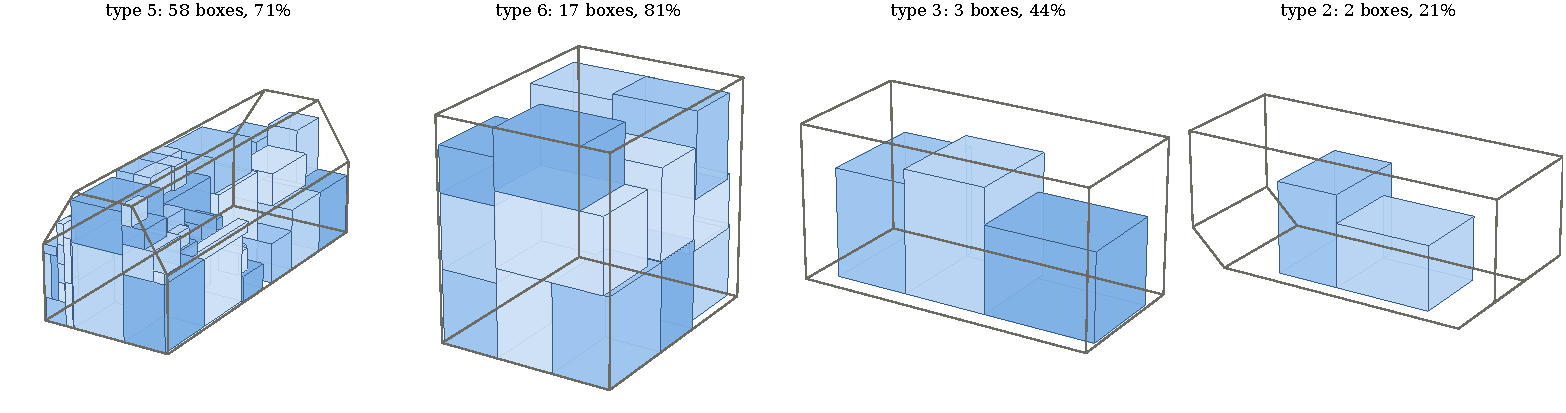
\includegraphics[width=\textwidth]{figures/loading.pdf}

\medskip
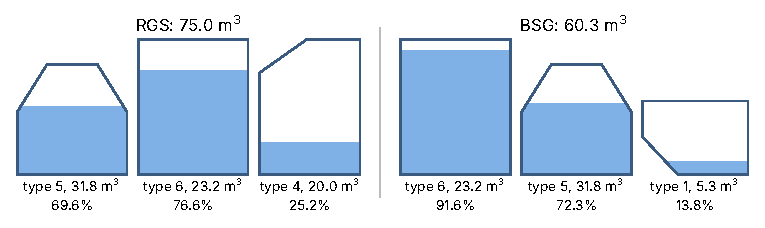
\includegraphics[width=\textwidth]{figures/liquid.pdf}
\caption{Solution of the instance with 80 boxes number 8 in the setting with one ULD of each
type ($t = 0.1$\,s): three ULDs (number of boxes and volume utilization) with a total volume of
60.3\,m$^3$, against 75.0\,m$^3$ for the ULDs of types 5, 6 and 4 of the RGS. Types 5 and 1 have
bevelled corners; the type 6 uses the substructure. The load of each ULD has been translated to
center its CoG, which is within range in the three ULDs. Fragile boxes are shown in orange.
Bottom: profile of the ULDs of both solutions filled up to their volume utilization, as if the
load were a liquid (the positions of the boxes of the RGS are not available).}
\label{fig:loading}
\end{figure}

\paragraph{Results by instance size.}
Tables~\ref{tab:size} and~\ref{tab:size2} report the total volume and the number of ULDs by
instance size. With $t = 1$\,s our algorithm uses less volume than the RGS in every group of
every setting, between 0.2\% and 16.6\% less. In the instances with 10 boxes, which fit in one
ULD, it uses more ULDs than the RGS (42--43 against 30) but less volume, since it splits the
boxes into two smaller ULDs when their total volume is smaller than that of one large ULD.

\begin{table}[htbp]
\centering
\small\setlength{\tabcolsep}{4pt}
\caption{Results by instance size in the Paquay setting (30 instances per size): total volume of
the ULDs (m$^3$) and number of ULDs ($|C|$) of the RGS and of BSG (mean of five runs).}
\label{tab:size}
\begin{tabular}{rrrrrrrr}
\toprule
 & \multicolumn{4}{c}{Volume of the ULDs (m$^3$)} & \multicolumn{3}{c}{$|C|$} \\
\cmidrule(lr){2-5}\cmidrule(lr){6-8}
$|I|$ & RGS & $t = 0.1$\,s & $t = 1$\,s & vs RGS & RGS & $t = 0.1$\,s & $t = 1$\,s \\
\midrule
10 & 502.4 & 450.2 & 442.3 & $-$12.0\% & 30 & 43 & 42 \\
20 & 880.7 & 851.7 & 820.6 & $-$6.8\% & 35 & 38.2 & 41 \\
30 & 1128.5 & 1121.6 & 1034.4 & $-$8.3\% & 47 & 55.8 & 51 \\
40 & 1485.5 & 1520.3 & 1431.4 & $-$3.6\% & 60 & 72 & 68.6 \\
50 & 1735.4 & 1753.2 & 1674.3 & $-$3.5\% & 66 & 75.6 & 73 \\
60 & 2073.7 & 2024.7 & 1916.1 & $-$7.6\% & 80 & 81.2 & 72 \\
70 & 2278.5 & 2210.1 & 2188.7 & $-$3.9\% & 82 & 94 & 88 \\
80 & 2552.1 & 2503.4 & 2357.8 & $-$7.6\% & 93 & 95.4 & 88.4 \\
90 & 2805.4 & 2686.7 & 2623.7 & $-$6.5\% & 102 & 111.2 & 104 \\
100 & 3205.2 & 2984.3 & 2827.7 & $-$11.8\% & 113 & 111.2 & 104.6 \\
\bottomrule
\end{tabular}
\end{table}

\begin{table}[htbp]
\centering
\small\setlength{\tabcolsep}{4pt}
\caption{Results by instance size in the adapted settings (30 instances per size; see
Table~\ref{tab:size}).}
\label{tab:size2}
\begin{tabular}{lrrrrrrrr}
\toprule
 & & \multicolumn{4}{c}{Volume of the ULDs (m$^3$)} & \multicolumn{3}{c}{$|C|$} \\
\cmidrule(lr){3-6}\cmidrule(lr){7-9}
 & $|I|$ & RGS & $t = 0.1$\,s & $t = 1$\,s & vs RGS & RGS & $t = 0.1$\,s & $t = 1$\,s \\
\midrule
\multirow{10}{*}{Adapted} & 10 & 497.3 & 433.0 & 433.0 & $-$12.9\% & 30 & 43 & 43 \\
 & 20 & 786.6 & 821.6 & 784.9 & $-$0.2\% & 33 & 38 & 35 \\
 & 30 & 1034.3 & 946.5 & 862.6 & $-$16.6\% & 45 & 45.2 & 39 \\
 & 40 & 1341.3 & 1324.4 & 1214.6 & $-$9.4\% & 57 & 65.8 & 64 \\
 & 50 & 1557.0 & 1555.1 & 1507.2 & $-$3.2\% & 60 & 70.8 & 63 \\
 & 60 & 1868.1 & 1813.1 & 1788.9 & $-$4.2\% & 72 & 76.8 & 73 \\
 & 70 & 2107.7 & 2002.9 & 1870.9 & $-$11.2\% & 78 & 86 & 86.8 \\
 & 80 & 2350.8 & 2244.0 & 2142.6 & $-$8.9\% & 86 & 92.2 & 91 \\
 & 90 & 2533.6 & 2392.8 & 2311.0 & $-$8.8\% & 92 & 103.8 & 90 \\
 & 100 & 2766.1 & 2669.2 & 2545.8 & $-$8.0\% & 100 & 104.2 & 104.2 \\
\midrule
\multirow{10}{*}{One} & 10 & 497.3 & 446.8 & 444.5 & $-$10.6\% & 30 & 42 & 43 \\
 & 20 & 786.6 & 804.8 & 768.7 & $-$2.3\% & 33 & 38 & 34 \\
 & 30 & 1034.3 & 979.0 & 866.8 & $-$16.2\% & 45 & 44 & 38 \\
 & 40 & 1341.3 & 1260.2 & 1165.9 & $-$13.1\% & 57 & 66.8 & 63 \\
 & 50 & 1538.2 & 1457.7 & 1372.1 & $-$10.8\% & 62 & 69 & 61 \\
 & 60 & 1825.7 & 1798.6 & 1740.4 & $-$4.7\% & 77 & 78 & 75.4 \\
 & 70 & 1996.6 & 1956.0 & 1873.7 & $-$6.2\% & 85 & 93 & 86 \\
 & 80 & 2192.9 & 2129.0 & 2088.8 & $-$4.7\% & 97 & 97.2 & 98 \\
 & 90 & 2358.6 & 2284.7 & 2225.1 & $-$5.7\% & 109 & 103.4 & 103 \\
 & 100 & 2594.2 & 2505.4 & 2462.1 & $-$5.1\% & 134 & 127.4 & 126.8 \\
\bottomrule
\end{tabular}
\end{table}

\subsection{Running time}
\label{sec:exp-time}

With $t = 0.1$\,s our algorithm takes 0.56--1.02\,s per instance on average (at most 8\,s),
and with $t = 1$\,s 3.5--6.8\,s (at most 54\,s). The RGS takes 0.19--0.42\,s per instance on
an Apple M2 Pro, about 0.5--1.1\,s on our processor once its single-thread speed, about 2.5
times ours according to PassMark \citep{PassMark}, is taken into account. Figure~\ref{fig:time}
shows how the volume changes with the time limit. At the time of the
RGS our algorithm already uses about 2--5\% less volume, and the difference grows with the time
limit, up to 8--9\% with $t = 2$\,s; with a very short time limit ($t = 0.02$\,s) it is
slightly worse than the RGS. With one ULD of each type, the unloaded volume goes from 43.6\,m$^3$
with $t = 0.02$\,s to 11.5\,m$^3$ with $t = 2$\,s, and is below that of the RGS (25.9\,m$^3$) from
$t = 0.05$\,s on. Giving the improvement phases the same time limit as the
construction, instead of $0.1\,t$, gives better solutions for the same $t$ but at a much higher
running time: up to about 10\,s per instance, the default is better at the same running time
(Figure~\ref{fig:time}, Paquay setting).


\begin{figure}[htbp]
\centering
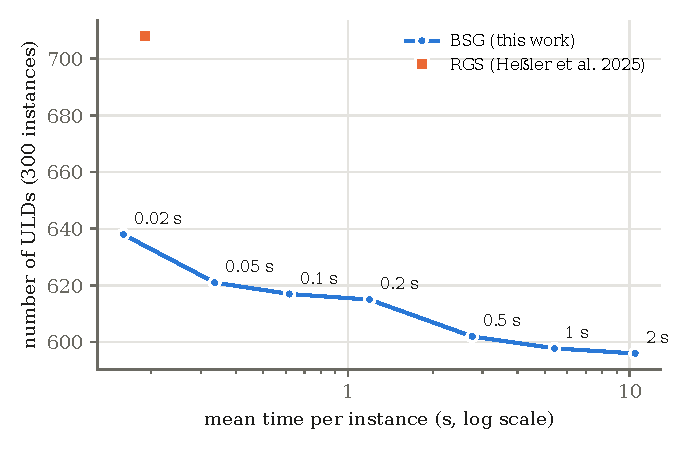
\includegraphics[width=\textwidth]{figures/time.pdf}
\caption{Volume of the ULDs relative to the RGS of \citet{Hessler2025} as a function of the mean
time per instance (the labels are time limits $t$; mean of five runs for 0.1\,s and 1\,s, one
run otherwise). The RGS is shown at its time on the Apple M2 Pro (filled square) and scaled to
our processor by the single-thread speed ratio of 2.53 (empty square). In the Paquay setting,
the dotted line gives the improvement phases the same time limit $t$ as the construction.}
\label{fig:time}
\end{figure}

\subsection{Contribution of the components}
\label{sec:exp-ablation}

Table~\ref{tab:ablation} reports the results with $t = 0.1$\,s when one component of the
algorithm is removed (one run; the complete algorithm is the mean of five runs, whose volume
varies by about 0.2\%).

\begin{table}[htbp]
\centering
\footnotesize\setlength{\tabcolsep}{3.5pt}
\caption{Ablation ($t = 0.1$\,s): volume of the ULDs relative to the RGS, ULDs with the CoG out
of range in the length or width direction and, with one ULD of each type, unloaded volume
(m$^3$). In bold, the measures that get clearly worse than with the complete algorithm. Basic BSG:
rule of \citet{Hessler2025}, spaces anchored at the nearest corner of the ULD, no substructure,
no restarts and no reduction phase.}
\label{tab:ablation}
\begin{tabular}{lrrrrrrr}
\toprule
 & \multicolumn{2}{c}{Paquay} & \multicolumn{2}{c}{Adapted} & \multicolumn{3}{c}{One} \\
\cmidrule(lr){2-3}\cmidrule(lr){4-5}\cmidrule(lr){6-8}
Variant & Vol. & CoG & Vol. & CoG & Vol. & Unl. & CoG \\
\midrule
Complete algorithm & $-$2.9\% & 7.8 & $-$3.8\% & 3 & $-$3.4\% & 22.8 & 5 \\
\midrule
No CoG penalty ($\lambda = 0$) & $-$6.0\% & \textbf{460} & $-$3.0\% & \textbf{281} & \textbf{$-$2.0\%} & 15.4 & \textbf{308} \\
No translation of the load & \textbf{$-$1.4\%} & \textbf{183} & $-$2.4\% & \textbf{117} & $-$2.7\% & 16.1 & \textbf{192} \\
Single-box blocks ($N_{\max} = 1$) & $-$2.7\% & \textbf{16} & \textbf{$-$2.4\%} & 4 & $-$3.0\% & 24.4 & 2 \\
No substructure & -- & -- & \textbf{$-$2.2\%} & 7 & \textbf{$-$1.7\%} & \textbf{33.0} & 14 \\
No restarts & -- & -- & -- & -- & $-$3.3\% & \textbf{38.3} & 5 \\
No priority in BSG ($\omega = 0$) & -- & -- & -- & -- & $-$8.0\% & \textbf{259.5} & 5 \\
Rule of \citet{Hessler2025} (no $\theta$) & $-$2.5\% & 7 & $-$3.6\% & 3 & $-$3.6\% & 25.0 & 5 \\
\midrule
No \textsc{Insert} & \textbf{$+$0.2\%} & 10 & \textbf{$+$0.2\%} & 4 & \textbf{$-$2.0\%} & 24.8 & 7 \\
Reduction with one new ULD & \textbf{$-$1.6\%} & 8 & \textbf{$-$2.5\%} & 2 & $-$3.0\% & 22.8 & 5 \\
No reduction phase & \textbf{$+$0.8\%} & 10 & \textbf{$+$0.6\%} & 2 & \textbf{$-$1.8\%} & 22.8 & 6 \\
\midrule
Basic BSG & \textbf{$+$13.9\%} & \textbf{90} & \textbf{$+$18.4\%} & \textbf{61} & \textbf{$+$9.4\%} & \textbf{54.6} & \textbf{59} \\
\bottomrule
\end{tabular}
\end{table}

The reduction phase is the component that makes the difference with the RGS: without it, or
without \textsc{Insert}, the volume is about the same as that of the RGS in the Paquay and adapted
settings, and loading the leftover boxes into two new ULDs instead of one saves a further
0.4--1.3 points. The CoG penalty $\lambda$ and the translation of the load keep the CoG in range:
without either of them, 117--460 ULDs violate the constraint. Without the penalty the volume
decreases in the Paquay setting, where the CoG limit of 5\% is very strict, and increases in the
other two; without the translation it increases in the three settings, since the penalty then
rejects loadings that a translation would have balanced. Building the load with blocks of
several boxes instead of single boxes reduces the volume by 1.4 points in the adapted setting and
by less elsewhere, halves the CoG violations in the Paquay setting and reduces the unloaded volume
with one ULD of each type: these boxes are highly heterogeneous, and few identical boxes can be
grouped. The substructure saves 1.6--1.7 points in the adapted settings. With one ULD of each type, the
priority of the boxes that fit in no other available ULD is essential: without it ($\omega = 0$),
259.5\,m$^3$ remain unloaded, which also explains the smaller volume of the ULDs; the restarts
reduce the unloaded volume from 38.3 to 22.8\,m$^3$. The choice of the ULD type with $\theta$
changes the volume by less than half a point in this run (0.8 points in the Paquay setting in a
run with $t = 0.05$\,s), and with one ULD of each type it reduces the unloaded volume from 25.0 to
22.8\,m$^3$: with an unlimited number of ULDs, a poor choice during the construction is mostly
corrected by the reduction phase.

Other variants did not improve the algorithm at the same running time: penalizing the CoG
excess in the evaluation of the blocks (its effect on the volume changed sign between runs),
anchoring the spaces at the nearest corner of the ULD (less volume in the Paquay setting, but
with 50\% more time, at which a larger $t$ is better), reloading each ULD from scratch or with
priority in \textsc{Insert}, eliminating ULDs without replacing them, and choosing the type of
each ULD by completing the solution with a fast construction (a rollout).

\subsection{Volume of the ULDs versus weight distribution}
\label{sec:exp-tradeoff}

Table~\ref{tab:lambda} shows the effect of the penalty $\lambda$ of the CoG excess. With
$\lambda = 0$ the CoG is ignored and 279--462 ULDs violate the constraint; any $\lambda \ge 0.5$
reduces the violations to at most 20 ULDs, and $\lambda \ge 2$ to at most 7, with a volume that
changes by at most 1.6 points. The constraint can therefore be enforced almost completely at a
small cost in volume, and the tuned value $\lambda = 1.4$ lies in this flat region.

\begin{table}[htbp]
\centering
\small
\caption{Effect of the CoG penalty $\lambda$ ($t = 0.1$\,s, one run; $\lambda = 1.4$ is the
complete algorithm, mean of five runs): volume of the ULDs relative to the RGS and ULDs with the
CoG out of range in the length or width direction.}
\label{tab:lambda}
\begin{tabular}{rrrrrrr}
\toprule
 & \multicolumn{2}{c}{Paquay} & \multicolumn{2}{c}{Adapted} & \multicolumn{2}{c}{One} \\
\cmidrule(lr){2-3}\cmidrule(lr){4-5}\cmidrule(lr){6-7}
$\lambda$ & Vol. & CoG & Vol. & CoG & Vol. & CoG \\
\midrule
0 & $-$6.0\% & 462 & $-$3.0\% & 279 & $-$2.1\% & 306 \\
0.5 & $-$3.3\% & 20 & $-$4.4\% & 8 & $-$3.3\% & 17 \\
1 & $-$2.2\% & 14 & $-$4.0\% & 5 & $-$3.3\% & 11 \\
1.4 & $-$2.9\% & 7.8 & $-$3.8\% & 3 & $-$3.4\% & 5 \\
2 & $-$3.5\% & 7 & $-$3.5\% & 1 & $-$3.2\% & 1 \\
5 & $-$3.7\% & 6 & $-$3.7\% & 0 & $-$3.4\% & 2 \\
30 & $-$3.8\% & 6 & $-$4.0\% & 0 & $-$3.4\% & 0 \\
\bottomrule
\end{tabular}
\end{table}
